\chapter{Introduction}
\label{cap:introduction}

This chapter introduces the fundamental aspects of the project to provide context for the work carried out. The following sections detail the two pillars of the proposal: the context of indoor climbing in climbing gyms and the use of gamification techniques applied to sports. Once these two main aspects are introduced, both the motivation and the primary objectives of this project are described. Finally, the structure of the rest of the document is outlined.

\section{Context of indoor climbing}

Climbing is a sport with numerous modalities, of which we will focus on indoor climbing, practiced in climbing gyms. Its main characteristics, route types, and difficulty systems are detailed below.

\subsection{How indoor climbing works}

A climbing gym is a sports facility that emulates natural rock climbing through artificial walls equipped with holds of different shapes, sizes, and colors. The climber's objective is to ascend a predefined route using exclusively the holds designated for that route. Routes are identified by holds of the same color. Each route has a starting point and an end point or \textit{top} (the final hold that must be grabbed with both hands to complete the ascent).

Unlike natural rock climbing, routes in climbing gyms are dynamic. That is, in order to provide variety and new challenges to climbers, the routes are periodically renewed. This task is carried out by route setters, professionals in charge of designing and setting the new boulders and routes.

\subsection{Types of routes in climbing gyms}

The main modalities practiced in a climbing gym are bouldering and sport climbing:

\begin{enumerate}
	\item \textbf{Bouldering.} It is practiced on low-height walls, usually up to 4 or 5 meters, with crash pads for safety, as can be seen in figure \ref{fig:imagen_bloque}. The objective of these types of routes is to find a solution to problems with short and intense movement sequences.

	\begin{figure}[h]
    \centering
    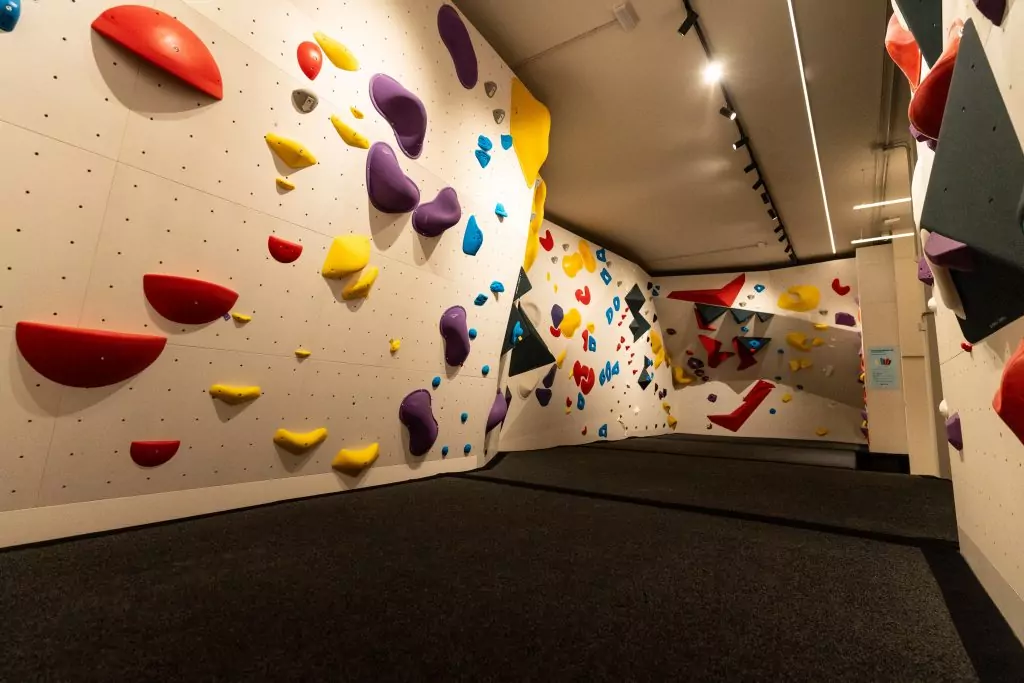
\includegraphics[width=0.6\textwidth]{./Imagenes/Fuentes/bloqueUadi.png} 
    \caption{Bouldering wall at UADIBLOC}
    \label{fig:imagen_bloque}
	\end{figure}

	\item \textbf{Sport climbing.} It is performed on taller walls, as can be seen in figure \ref{fig:imagen_via}, requiring safety equipment such as a rope, a harness, and a belay system. In these types of routes, climbers must complete long paths where endurance and effort management predominate. During the ascent, the climber clips the rope into intermediate anchors, and the belayer, from the ground, controls the rope to arrest any potential falls.
\end{enumerate}

\begin{figure}[h]
    \centering
    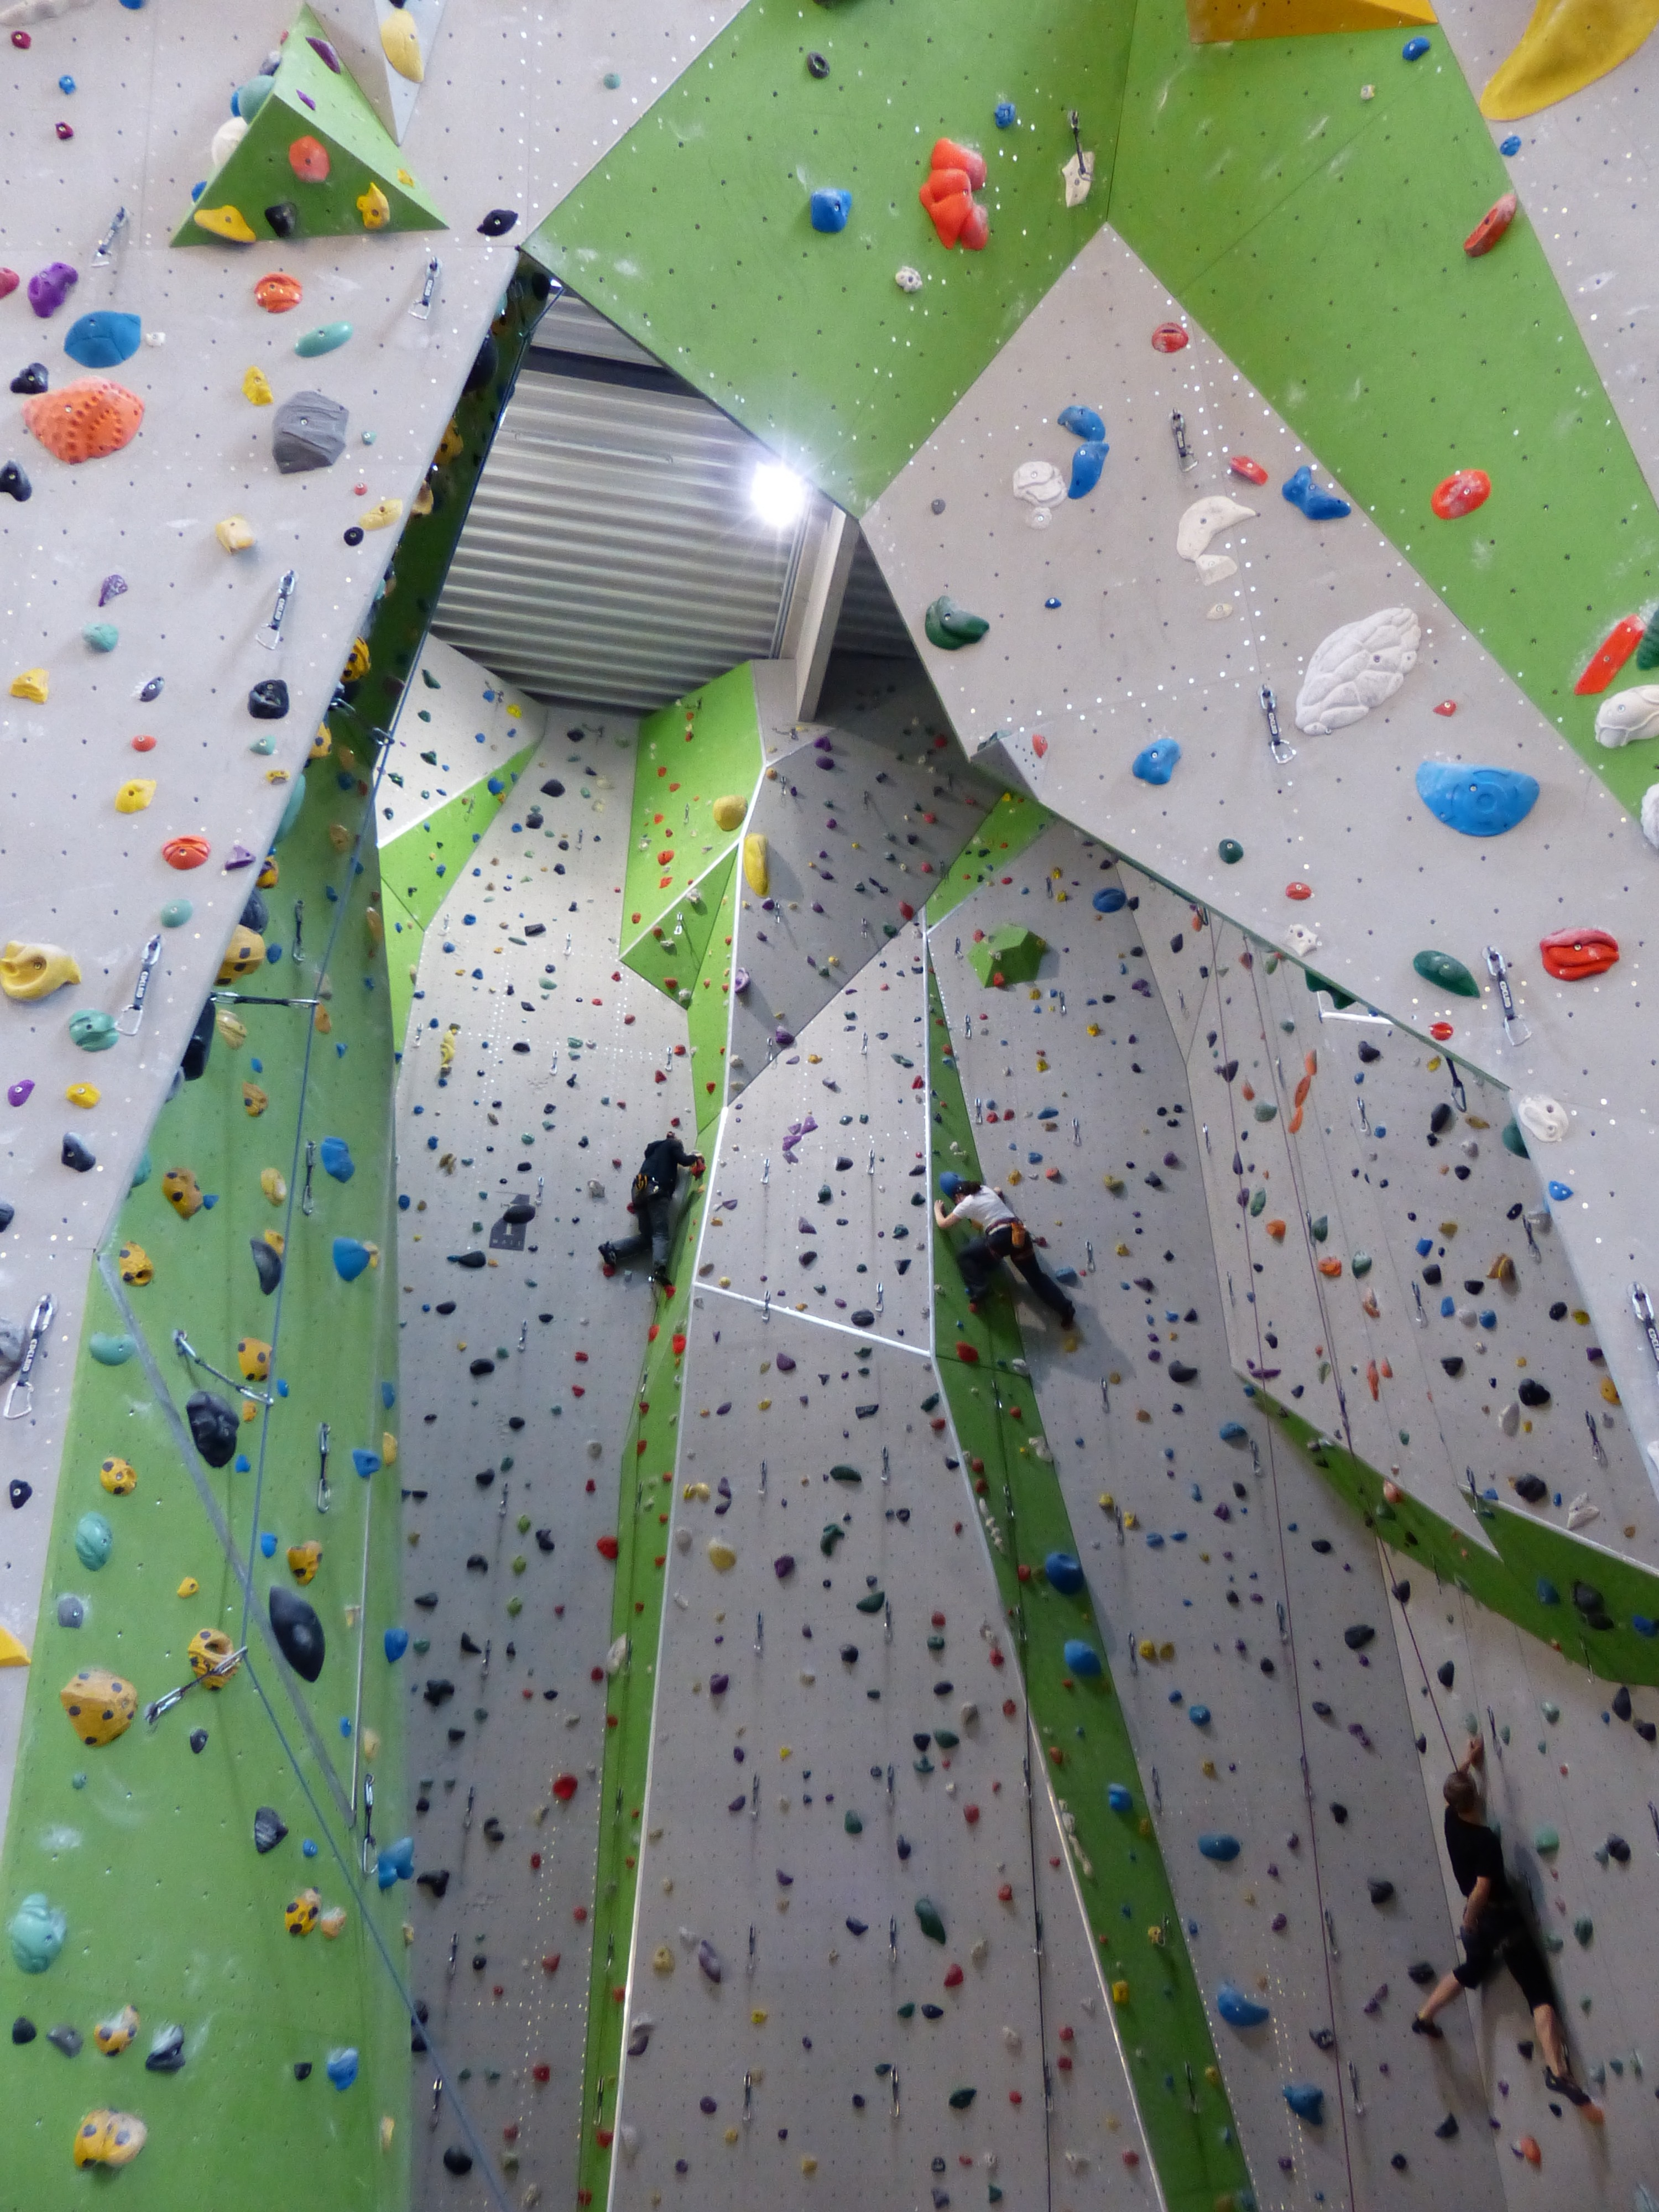
\includegraphics[width=0.6\textwidth]{./Imagenes/Fuentes/via.jpg} 
    \caption{Sport climbing routes in a gym}
    \label{fig:imagen_via}
\end{figure}

\subsection{Difficulty and progress}

To encourage and facilitate progress in the activities of climbers, it is common for each route, both boulder and sport, to be assigned a difficulty grade that allows estimating the required level to complete it. This grade is usually indicated on a tag placed on the starting hold or area of the route. 

Although there are various scales to measure progress, bouldering predominantly uses the Fontainebleau scale, and the French scale is the most common for sport climbing. These scales will be further detailed in chapter \ref{cap:estadoDelArte}.

In addition to these standard scales, many climbing gyms use internal color-based systems to associate difficulty ranges to each route. These color circuits usually group official grades into broader ranges. This system has a direct relationship with standard scales, but it is particularly useful and important because it reduces the technical entry barrier for beginners, enables a quick reading of the level on the wall, and serves as a strong visual motivation element by allowing climbers to clearly perceive their progress.

\section{Context of gamification in sports}

Gamification is defined as the use of game mechanics, elements, and design principles in non-game contexts \citep{deterding2011game}. While standard gamification is oriented towards a general playful environment, when applied to sports activities, its mechanics are adapted and tailored to focus on training. In this sense, gamification techniques applied to sports activities usually focus on fostering and increasing the athlete's motivation, improving user retention, and promoting long-term adherence to the practice.

\subsection{RAMP psychological model}

One of the main foundations for designing motivating gamified experiences is the RAMP psychological model (\textit{Relatedness, Autonomy, Mastery, Purpose}) proposed by Marczewski \citep{marczewski2015even}, which is aligned with the classic theories of intrinsic motivation defined in \cite{ryan2000self}. This model highlights four main user needs:

\begin{itemize}
	\item \textbf{Relatedness:} the user's need to have social connections, recognition, and a sense of belonging to a community.
	\item \textbf{Autonomy:} the user's need to feel in control and make decisions to progress.
	\item \textbf{Mastery:} the need to feel continuous improvement through achievable and progressive goals.
	\item \textbf{Purpose:} the need to feel that the effort has a meaning beyond the immediate task.
\end{itemize}

\subsection{The PBL system (\textit{Points, Badges, Leaderboards})}

Based on the RAMP model and reward mechanics, the PBL system emerges \citep{marczewski2013pbl}. This is a classic gamification implementation that grounds motivational concepts and consists of three main elements:

\begin{itemize}
	\item \textbf{Points:} represent the user's effort or performance (for example, difficulty climbed, number of attempts, or consistency).
	\item \textbf{Badges:} represent achievements reached and visualize the athlete's evolution (for example, completing 100 routes or achieving your first 7A difficulty route).
	\item \textbf{Leaderboards:} compare results among users, encouraging healthy competition and a sense of community.
\end{itemize}

\subsection{Benefits of gamification in sports}

The integration of gamification mechanics in health and sports applications brings highly relevant benefits \citep{koivisto2019rise}:

\begin{itemize}
	\item \textbf{Higher retention:} constant feedback reduces dropout rates and improves training consistency.
	\item \textbf{Progress visualization:} data tracking allows visualizing evolution through metrics and tangible achievements.
	\item \textbf{Community reinforcement:} social interactions increase user engagement with the sport and their surroundings.
\end{itemize}

In an individual sport like climbing, where physical progress is often slow and long plateaus exist, these mechanics are especially useful for maintaining the athlete's motivation and consistency.

\section{Motivation of this work}

Climbing is an individual sport where tracking progress is usually done manually (notebooks, memory, or generic external applications not integrated into the dynamics of the climbing gym itself). 

The main general objective is to promote the sport of climbing by facilitating the tracking and guidance of athletes in their different activities, motivating them to continue practicing it through gamification techniques. Likewise, as a secondary general objective, it provides a tool that allows digitizing climbing activities for sports centers that adopt this solution, adding a unique value to their sports offerings.

More specifically, the aim of this work is to create a solution that allows logging completed routes specific to each climbing gym, preserving the activity history to analyze the user's evolution. Additionally, the solution incorporates gamification elements such as statistics and \textit{Leaderboards} to transform training into a more social and motivating experience, favoring consistency and healthy competition among the local climbing community.

We highlight the need to approach this project from a User-Centered Design (UCD) perspective by placing the users' needs, frustrations, and expectations at the center of the process, with the goal that the finally developed solution meets the real needs of the users and, therefore, provides real value.

\section{Objectives}

This section defines the objectives that guide the project's development, making a distinction between general and specific objectives.

\subsection{General objective}

Develop a web application compatible with mobile devices that, on the one hand, promotes the practice of climbing by facilitating user tracking and motivation through gamification; and on the other hand, digitizes the sports management of climbing gyms.

\subsection{Specific objectives}

\begin{enumerate}
	\item Develop a tracking system for climbers that allows managing their personal profile, their statistics, and easily logging the status of their routes (marking whether they have been flashed, completed, or are an ongoing project).
	\item Incorporate gamification mechanics (PBL system) aimed at improving long-term user motivation.
	\item Develop a route management system for \textit{route setters} to minimize the effort required to log changes and new sets in the climbing gym.
	\item Implement social features (friendships, progress comparison, and statistics) to encourage healthy competition and a sense of belonging to the community.
	\item Design a simple, intuitive, and efficient user interface and user experience, prepared for users with varying levels of technological skill.
\end{enumerate}

\section{Document structure}

This document is organized into nine chapters detailing the entire process of planning, design, application development, and user testing and validation. The content of each is briefly summarized below:

\begin{itemize}
    \item \textbf{Chapter~\ref{cap:introduccion}: Introduction.} Presents the context of \textit{indoor} climbing, the fundamentals of sports gamification, and the motivation and objectives of the work.
    \item \textbf{Chapter~\ref{cap:estadoDelArte}: State of the Art.} Contextualizes the boom in climbing along with its difficulty systems, and analyzes applications in the sector and other sports to identify the current limitations upon which the solution is based.
    \item \textbf{Chapter~\ref{cap:metodologiaDesarrollo}: Development Methodology and Planning.} Details the Scrumban framework, the tools used, and the role of artificial intelligence as development support.
    \item \textbf{Chapter~\ref{cap:analisisRequisitos}: Requirements Analysis and Specification.} Defines user roles and key functionalities through user stories.
    \item \textbf{Chapter~\ref{cap:disenoSistema}: System Design and Technical Decisions.} Outlines the technology \textit{stack}, system architecture (\textit{backend} and \textit{frontend}), database design, and user interface.
    \item \textbf{Chapter~\ref{cap:implementacion}: Implementation and Development.} Describes the development process of the \textit{software} components and the technical challenges overcome.
    \item \textbf{Chapter~\ref{cap:cicd}: Continuous Integration, Deployment, and DevOps.} Explains the setup of the CI/CD \textit{pipeline}, infrastructure management, and the publishing process on Google Play.
    \item \textbf{Chapter~\ref{cap:pruebasValidacion}: Testing and Validation.} Covers the testing strategy and the results of the validation sessions with real users.
    \item \textbf{Chapter~\ref{cap:conclusiones}: Conclusions and Future Work.} Determines the obtained results, evaluates the fulfillment of the defined objectives, and proposes a series of tasks for the future evolution of the project.
\end{itemize}

Finally, this document concludes with the personal contributions of the authors, the consulted bibliography, and the corresponding appendices.